\section{Methodology}
\label{S:w3}
Here we develop a machine learning framework for mode detection that is specifically tailored to exploit the large, ubiquitous, low-cost, noisy, and partially labelled Wi-Fi data available in our case study. We use a semi-supervised residual net (ResNet) for developing very deep neural networks that are based on Multilayer Perceptron (MLP). \cref{fig:Resarch} depicts the general working of the proposed framework. After extracting labelled and unlabelled data, a ResNet MLP classifier is trained using solely labelled data. The trained classifier is then used to predict the mode of transportation of a sample of unlabelled data. In the next step, predicted modes are used as the labels for the selected sample, known as \textit{Pseudo-labels}. Next, ResNet MLP classifier is re-trained on labelled data and pseudo-labelled data. The classifier is retrained on other portions of unlabelled data, and in the end, the accuracy of the method is evaluated on a labelled validation set.

In this study, the ResNet MLP architecture is developed and implemented as the classifier in the pseudo-labelling algorithm. In short, the classifier consists of an input layer, multiple building blocks, and an output layer. Each building block consists of two or three fully connected layers, with an identity shortcut connection that skips these layers.  

The proposed method in this research aims at addressing two challenging issues in related studies~\cite{he2016deep,lee2013pseudo}:
\begin{enumerate}
    \item[a.] Lowering the associated costs of data collection by incorporating a large amount of unlabelled data within the semi-supervised framework
    \item[b.] Benefiting from the large number of layers in a very deep network, without suffering from vanishing gradient problem, by implementing identity shortcut connection, derived from ResNet architecture
\end{enumerate}
In this section, we first describe ResNet and the way we developed our neural network using it. Pseudo-label, a simple, yet efficient semi-supervised learning method that we are applying to the core architecture is then discussed.

\subsection{ResNet-based MLP}
Deep Residual Network (ResNet) was originally introduced for image recognition and won the first place at the ILSVRC 2015 classification task \cite{he2016deep}. Although ResNet has been mainly implemented in convolutional neural networks, the idea of using \textit{identity shortcut connections} to skip one or more layers can be applied to other types of networks. In this study, we exploit this idea to develop a very deep multilayer perceptron.

The ResNet MLP developed for this study consists of three types of layers discussed below:
\begin{itemize}
    \item \textbf{Input Layer:} 15 features are extracted from raw labelled and unlabelled data. For each trip, values of features are normalized and inserted into the 15-node input layer.
    \item \textbf{Building Block:}
    A building block, or residual blocks, consists of a few fully connected layers and identity shortcuts. Finding adequate number of building blocks, and number of layers in each block, requires testing different networks and comparing the results.
    Feeding a block with input $x$, the output of the building block is \cite{he2016deep}:
    \begin{equation}
    \label{eq1}
        y= f(x,\{w_i\})+x
    \end{equation}
    in which $f$ is a shallow MLP, with two or three fully connected layers. For instance, in a two layer building block, $f$ can be written as:
    \begin{equation}
        f(x,\{w_1,w_2\})= W_2\sigma(W_1x) 
    \end{equation}
    Here $\sigma$ is the activation function, which is selected to be ReLU \cite{nair2010rectified}, similar to the original paper \cite{he2016deep}. 
    \item \textbf{Output Layer:} It consists of three nodes, for three modes of transportation investigated in our study. Similar to other layers in the network, output layer is fully connected. The outputs from previous layers are inserted into the last fully connected layer for classification. Softmax activation function is used to create probability distribution for three transportation modes.
\end{itemize}

\begin{center}
\begin{figure*}
  \centering
  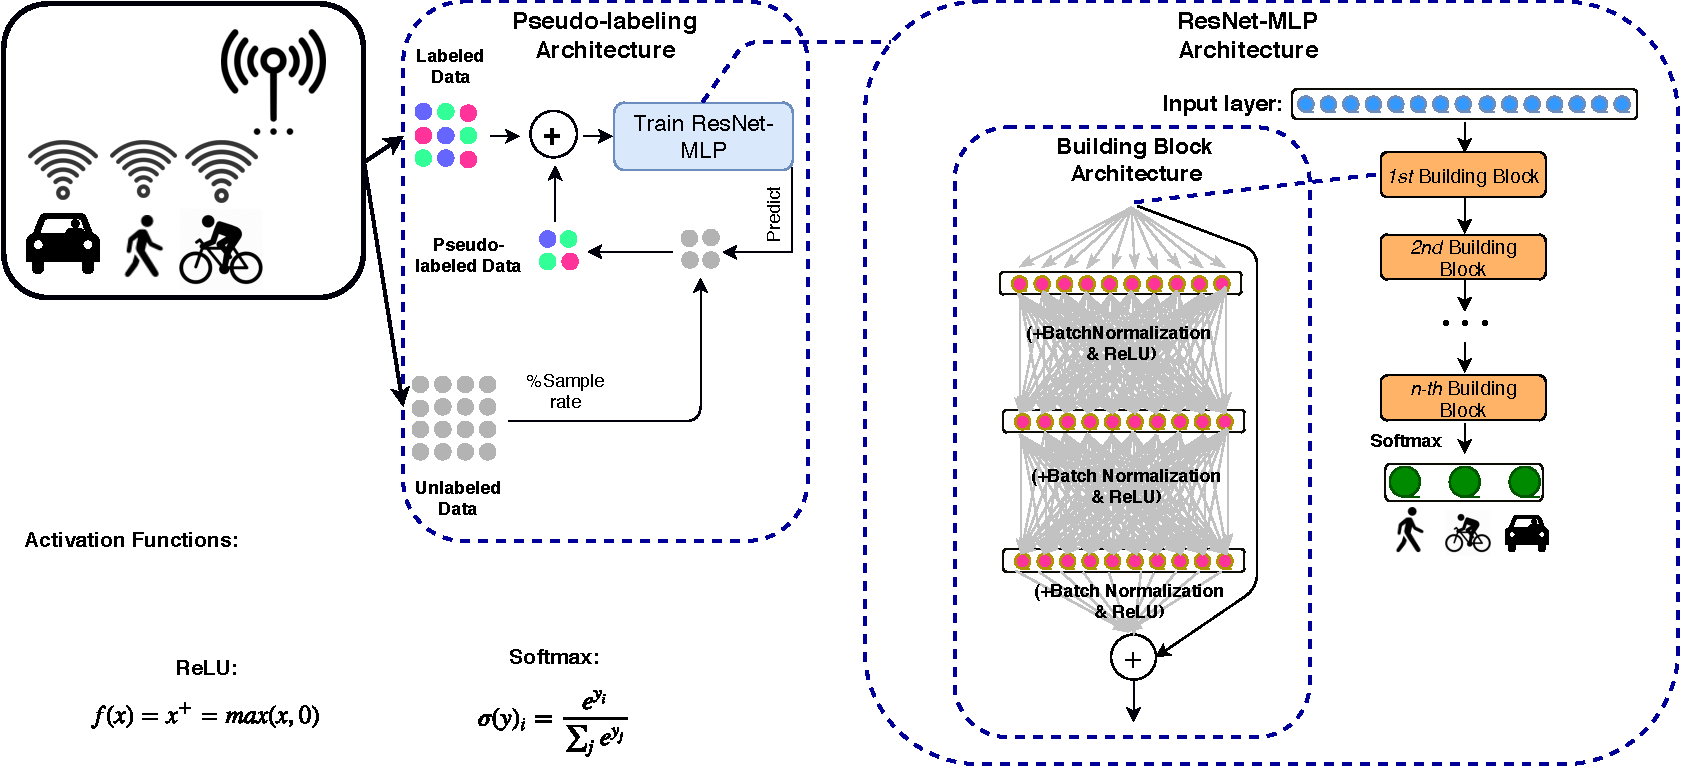
\includegraphics[scale=0.5]{chapter_2/figures/ResArch.pdf}% trim=left bottom right top
  \caption{Conceptual framework}
  \label{fig:Resarch}
\end{figure*}
\end{center}

By adding the output of shortcut connections to that of the stacked layers in equation \ref{eq1}, optimization of the network becomes easier, with no additional parameters or computational burden added \cite{he2016deep,he2016identity}. 

\subsection{Pseudo-Label}
Semi-supervised learning techniques are implemented to reduce the reliance on large amounts of expensive labelled data required in supervised learning algorithms. Unlabelled data are easy to collect in large volumes with lower costs compared to labelled datasets. In this study, a simple, yet efficient method for semi-supervised learning, called pseudo-label, is utilized \cite{lee2013pseudo}. 

In each iteration of the algorithm, pseudo-labels are defined as the classes with maximum predicted probability for each unlabelled sample.
The ResNet MLP network is trained on labelled and pseudo-labelled data in a supervised fashion. In every weight update, pseudo-labels are recalculated and are used in the loss function. The overall loss function of the learning task is written as \cite{lee2013pseudo}: 
\begin{equation}
    L=\frac{1}{n}\sum_{i=1}^{n}\sum_{m=1}^{M}L(y_i^m,f_i^m)+\alpha(t)	\frac{1}{n\prime}\sum_{i=1}^{n\prime}\sum_{m=1}^{M}L(y\prime _i^m,f\prime _i^m)
\end{equation}
Here $n$ and $n\prime$ are the number of batches for labelled and unlabelled data, respectively; M is the number of classes i.e. modes of transportation investigated in our case; $y$ and $y'$ are labels and pseudo-labels respectively; $f$ and $f'$ are the network outputs of labelled and pseudo-labelled samples; and $\alpha(t)$ is the balancing coefficient \cite{lee2013pseudo}, or the weight of unlabelled loss on the value of overall loss function. Performance of the algorithm is affected by the value of $\alpha(t)$. In this study, we utilize the same \textit{deterministic annealing process} as in \cite{lee2013pseudo}, to determine the value of $\alpha$ between 0 and 3, ascending with the epoch number.

Pseudo-labelling is a relatively simple semi-supervised algorithm based on self-learning scheme, that may perform poorly when the accuracy in predicting unlabelled samples are low. However, the simplicity and easy implementation of the algorithm, along with relatively high performance of the ResNet MLP classifier on labelled data, led us to add the algorithm to our ResNet MLP classifier. 